%%%%%%%%%%%%%%%%%%%%%%%%%%%%%%%%%%%%%%%%%%%%%%%%%%%%%%%%%%%%%%%%%%%%%%%%%%%%%%%%%%%%%%%%%%%%%%%%%%%%%%%
%%%%%%%%%%%%%% Template de Artigo Adaptado para Trabalho de Diplomação do ICEI %%%%%%%%%%%%%%%%%%%%%%%%
%% codificação UTF-8 - Abntex - Latex -  							     %%
%% Autor:    Fábio Leandro Rodrigues Cordeiro  (fabioleandro@pucminas.br)                            %% 
%% Co-autor: Prof. João Paulo Domingos Silva, Harison da Silva e Anderson Carvalho                   %%
%% Revisores normas NBR (Padrão PUC Minas): Helenice Rego Cunha e Prof. Theldo Cruz                  %%
%% Versão: 1.1     18 de dezembro 2015                     	                                     %%
%%%%%%%%%%%%%%%%%%%%%%%%%%%%%%%%%%%%%%%%%%%%%%%%%%%%%%%%%%%%%%%%%%%%%%%%%%%%%%%%%%%%%%%%%%%%%%%%%%%%%%%


\documentclass[a4paper,12pt,Times]{article}
\usepackage{abakos}  %pacote com padrão da Abakos baseado no padrão da PUC

%%%%%%%%%%%%%%%%%%%%%%%%%%%
%Capa da revista
%%%%%%%%%%%%%%%%%%%%%%%%%%

%\setcounter{page}{80} %iniciar contador de pagina de valor especificado
\newcommand{\monog}{Projeto e Análise de Algoritmos}
\newcommand{\monogES}{Trabalho 1 - Escrita de programas eficientes}
\newcommand{\tipo}{Artigo}  % Especificar a seção tipo do trabalho: Artigo, Resumo, Tese, Dociê etc
\newcommand{\origem}{Brasil }
\newcommand{\editorial}{Belo Horizonte, p. 01-07, jun. 2023}  % p. xx-xx – páginas inicial-final do artigo
\newcommand{\lcc}{\scriptsize{Licença Creative Commons Attribution-NonCommercial-NoDerivs 3.0 Unported}}

%%%%%%%%%%%%%%%%%INFORMAÇÕES SOBRE AUTOR PRINCIPAL %%%%%%%%%%%%%%%%%%%%%%%%%%%%%%%
\newcommand{\AutorA}{Gabriel Sebe Lucchesi Barbosa}
\newcommand{\funcaoA}{}
\newcommand{\emailA}{1319971@sga.pucminas.br}
\newcommand{\cursA}{Aluno de Ciência da Computação}
\newcommand{\AutorB}{Guilherme Vedovelo de Britto Claro}
\newcommand{\funcaoB}{}
\newcommand{\emailB}{1331587@sga.pucminas.br}
\newcommand{\cursB}{Aluno de Ciência da Computação}
\newcommand{\AutorC}{Luiz Fernando Oliveira Maciel}
\newcommand{\funcaoC}{}
\newcommand{\emailC}{lfomaciel@sga.pucminas.br}
\newcommand{\cursC}{Aluno de Ciência da Computação}
% 
% Definir macros para o nome da Instituição, da Faculdade, etc.
\newcommand{\univ}{Pontifícia Universidade Católica de Minas Gerais}

\newcommand{\keyword}[1]{\textsf{#1}}

\begin{document}
% %%%%%%%%%%%%%%%%%%%%%%%%%%%%%%%%%%
% %% Pagina de titulo
% %%%%%%%%%%%%%%%%%%%%%%%%%%%%%%%%%%

\begin{center}

\includegraphics[scale=0.2]{figuras/brasao.jpg} \\
PONTIFÍCIA UNIVERSIDADE CATÓLICA DE MINAS GERAIS \\
Instituto de Ciências Exatas e de Informática

% \vspace{1.0cm}

\end{center}

 

\vspace{1.0cm}

\begin{flushright}
\singlespacing 
\normalsize{\AutorA \footnote{\funcaoA \cursA,  \emailA . }} \\
\normalsize{\AutorB \footnote{\funcaoB \cursB,  \emailB . }} \\
\normalsize{\AutorC \footnote{\funcaoC \cursC,  \emailC . }} \\
%\normalsize{\AutorD \footnote{\funcaD \cursD, \origem -- \emailD . }} \\
%deixar com o valor `0` e usar o '*' no inicio da frase
% \symbolfootnote[0]{Artigo recebido em 10 de julho de 1983 e aprovado em 29 de maio 2012}
\end{flushright}
\thispagestyle{empty}

\vspace{1.0cm}

\begin{abstract}
\noindent
Este trabalho consiste na implementação de dois algoritmos que solucionam o problema de otimização de uma rota de coleta e entrega de produtos entre diversas lojas, encontrando o caminho de menor custo.
\\\textbf{\keyword{Palavras-chave: }} Projeto e Análise de Algoritmos. Otimização. Python. Caixeiro Viajante.
\end{abstract}

%%%%%%%%%%%%%%%%%%%%%%%%%%%%%%%%%%%%%%%%%%%%%%%%%%%%%%%%%


\selectlanguage{brazilian}
 \onehalfspace  % espaçamento 1.5 entre linhas
 \setlength{\parindent}{1.25cm}

%%%%%%%%%%%%%%%%%%%%%%%%%%%%%%%%%%%%%%%%%%%%%%%%%
%% INICIO DO TEXTO
%%%%%%%%%%%%%%%%%%%%%%%%%%%%%%%%%%%%%%%%%%%%%%%%%

%%%%%%%%%%%%%%%%%%%%%%%%%%%%%%%%%%%%%%%%%%%%%%%%%%%%%%%%%%%%%%%%%%%%%%%%%%%%%%%%%%%%%%%%%%%%%%%%%%%%%%%
%%%%%%%%%%%%%% Template de Artigo Adaptado para Trabalho de Diplomação do ICEI %%%%%%%%%%%%%%%%%%%%%%%%
%% codificação UTF-8 - Abntex - Latex -  							     %%
%% Autor:    Fábio Leandro Rodrigues Cordeiro  (fabioleandro@pucminas.br)                            %% 
%% Co-autores: Prof. João Paulo Domingos Silva, Harison da Silva e Anderson Carvalho		     %%
%% Revisores normas NBR (Padrão PUC Minas): Helenice Rego Cunha e Prof. Theldo Cruz                  %%
%% Versão: 1.1     18 de dezembro 2015                                                               %%
%%%%%%%%%%%%%%%%%%%%%%%%%%%%%%%%%%%%%%%%%%%%%%%%%%%%%%%%%%%%%%%%%%%%%%%%%%%%%%%%%%%%%%%%%%%%%%%%%%%%%%%
\section{\esp Introdução}
Um caminho simples em um grafo direciado é um caminho sem repetição de vértices. Ou seja, um caminho simples é uma sequência de vértices e arestas sem repetir o mesmo vértice mais de uma vez.

\begin{center}
    
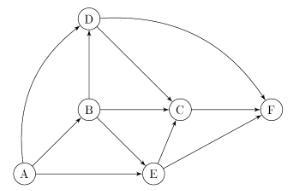
\includegraphics{figuras/grafodirecionado.png}

\end{center}

No gráfico acima, as sequências de vértices A, B, E, F e a sequência A, D, C, F são caminhos simples. Essas duas sequências também são caminhos disjuntos em arestas, pois não possuem arestas iguais entre si.

O problema de achar os caminhos disjuntos em arestas em um grafo possui vários usos em diversas áreas. Para isso, nós implementamos um algoritmo capaz de achar quantos e quais caminhos disjuntos existem em um grafo gerado de forma automática.

\section{\esp Resolução}
Para resolvermos o problema, inicialmente assumimos que todas as arestas no grafo possuem capacidade de fluxo unitária. Considerando que um grafo possua um número k máximo de caminhos disjuntos de um vértice s à um vértice t, podemos dizer que o fluxo máximo do vértice s ao vértice t será k (já que a capacidade de fluxo é unitária em todos as arestas). \cite{disjoint} Para encontrarmos o número máximo de caminhos disjuntos precisamos, portanto, apenas encontrar o fluxo máximo do grafo, e a partir do corte das arestas que possuem fluxo maior que 0 utilizarmos força bruta para encontrar um conjunto de caminhos disjuntos que possua o mesmo número de elementos que o valor máximo encontrado.

\section{\esp Implementação}

Nosso algoritmo foi desenvolvido em Python devido à sua alta abstração e consequente facilidade de implementação. Link do código-fonte: \url{https://github.com/lfnand0/Grafos-TP2}

Os grafos foram representados como matrizes de adjacência, onde a coluna representa o vértice de saída e a fileira o vértice de entrada, e o valor nessa posição é 1 caso exista uma aresta e 0 caso contrário.
Para encontrar o fluxo máximo, utilizamos o algoritmo de Edmonds-Karp \cite{10.5555/2168303}. Ao fim da execução do algoritmo, temos uma matriz com o fluxo residual - como precisamos apenas do corte onde existe fluxo, comparamos a matriz do grafo com o fluxo residual e geramos uma nova matriz (chamada de dif) seguindo as seguintes regras: para cada posição em uma matriz n x n: caso o valor seja 0 nessa posição na matriz do grafo, o elemento na posição na matriz dif será 0; caso seja 1, o elemento na matriz dif receberá o resultado da operação xor entre 1 e o elemento na matriz do fluxo residual. Visualização:

\begin{figure}[ht]
	\centering	
	\caption[\hspace{0.1cm}Grafo.]{Um grafo direcionado qualquer e sua matriz de adjacência}
	\vspace{-0.4cm}
	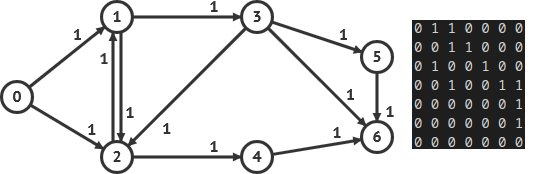
\includegraphics[width=0.6\textwidth]{figuras/grafo.png}
	 \vspace{-0.2cm}
	\label{fig:figura1}
\end{figure}
\vspace{-0.5cm}

\begin{figure}[ht]
	\centering	
	\caption[\hspace{0.1cm}Fluxo Residual.]{A matriz do fluxo residual do vértice 0 ao 6 encontrado após a execução do algoritmo de Edmonds-Karp}
	\vspace{-0.4cm}
	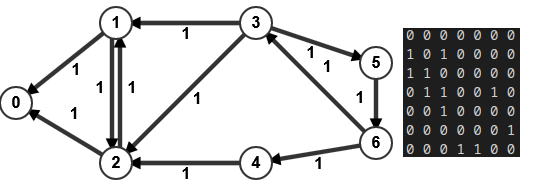
\includegraphics[width=0.6\textwidth]{figuras/fluxo.png}
	 \vspace{-0.2cm}
	\label{fig:figura2}
\end{figure}
\vspace{-0.5cm}

\begin{figure}[ht]
	\centering	
	\caption[\hspace{0.1cm}Fluxo Residual.]{A matriz "dif" encontrada após as operações explicadas acima}
	\vspace{-0.4cm}
	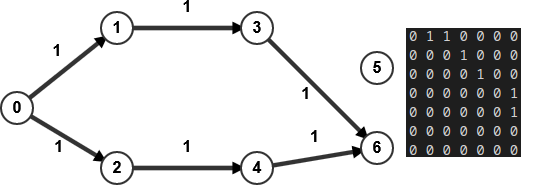
\includegraphics[width=0.6\textwidth]{figuras/dif.png}
	 \vspace{-0.2cm}
	\label{fig:figura3}
\end{figure}


Partindo dessa nova matriz "dif", realizamos primeiramente uma busca em profundidade, encontrando todos os caminhos do vértice origem ao destino e os salvando em uma lista. Depois criamos uma lista vazia chamada "disjuntos" para os caminhos disjuntos e "visitadas" para todas as arestas visitadas, e executamos o seguinte código:

\begin{center}	
         \textbf{Algoritmo 1 -  Encontrar conjunto de caminhos disjuntos}
	\vspace{-0.3cm}
\begin{minipage}[ht]{13cm}
\begin{algorithm}[H]
  \footnotesize
  \caption{Encontrar conjunto de caminhos disjuntos}
  \label{alg:rnagenerica}
  \begin{algorithmic}[1]
    \STATE Preenche o vetor de $attributes.size+1$ atributos com os valores dos atributos, sendo a primeira posição do vetor preenchida com o valor 1
		\STATE $hidden\_layer\_size =  attributes.size*2+1;$

    \FOR{caminhoA in caminhos}
        \STATE $disjuntos[] = [].append(caminhoA);$
        \STATE $visitadas = [].extend(caminhoA);$
        \FOR{$caminhoB$ en $caminhos - caminhoA$}
            \IF{$nenhuma aresta de caminhoB$ em $visitadas$}
                \STATE $disjuntos.append(caminhoB);$
                \STATE $visitadas.extend(caminhoB);$
            \ENDIF
        \ENDFOR
        \IF{$disjuntos.length$ == $maxflow$}
            \STATE return $disjuntos;$
        \ENDIF
    \ENDFOR
  \end{algorithmic}
\end{algorithm}
% \vspace{-0.3cm} % espaço entre algoritmo e fonte

\end{minipage}
\end{center}

Após a execução desse algoritmo, temos a lista com o conjunto de caminhos disjuntos.

\section{\esp Utilização do código}
Para utilizar o código, é necessário ter instalado o Python em uma versão igual ou superior à 3. Nosso código apresenta diversas flags para chamada inline, para que o usuário consiga utilizar da maneira que deseja. O usuário pode utilizar quantas e quais flags quiser. As flags que podem ser utilizadas são as seguintes: 

\subsection {\esp -prob [float]} 
A probabilidade que dois vértices tenham uma aresta em comum na geração de grafos aleatórios. Caso não seja utilizado a probabilidade será 0.3.

\textbf{Exemplo:} python tp2.py -prob 0.1

\subsection {\esp -arq [string]} 
Diretório de um arquivo txt com a matriz de adjacência de um grafo.

\textbf{Exemplo:} python tp2.py -arq "./grafos cíclicos/50.txt"

\subsection {\esp -ver [int]} 
Número de vértices a ser usado na geração de grafo. Caso não seja utilizado o número de vértices será 10.

\textbf{Exemplo:} python tp2.py -ver 100

\subsection {\esp -ori [int]}
Vértice de origem. Caso não seja utilizado, o vértice de origem será 0.

\textbf{Exemplo:} python tp2.py -ori 1

\subsection {\esp -des [int]}
Vértice de destino. Caso não seja utilizado, o vértice de destino será n - 1.

\textbf{Exemplo:} python tp2.py -des 9

\subsection {\esp -cam [string]} 
Diretório para salvar os caminhos disjuntos encontrados. Caso não seja utilizado, os caminhos serão salvos em "./disjuntos.txt"

\textbf{Exemplo:} python tp2.py -cam "./out/disj.txt"

\subsection {\esp -w [string]}
 Diretório para salvar o grafo gerado. Caso não seja utilizado o grafo gerado não será salvo
 
\textbf{Exemplo:} python tp2.py -w "./grafos simples/50.txt"

\subsection {\esp -ciclo}
Gera um grafo cíclico.

\textbf{Exemplo:} python tp2.py -ciclo

\subsection {\esp -completo}
Gera um grafo completo

\textbf{Exemplo:} python tp2.py -completo

\section{\esp Geração de Grafos Aleatórios}

Nosso algoritmo também é capaz de gerar grafos cíclicos, simples e completos de forma automática para serem testados pelo nosso método de busca de caminhos disjuntos em arestas.

Para a geração de grafos simples, utilizamos o Modelo Erdős–Rényi, que adiciona arestas ao grafo a partir de uma probabilidade definida.\cite{Erdos:1959:pmd}. Para grafos completos, chamamos a função que gera grafos simples, porém passando uma probabilidade de 1 (100\%) - ou seja, existe uma aresta saíndo de cada vértice do grafo para todos os outros. Para grafos cíclicos, apenas adicionamos uma aresta saíndo de um vértice e indo para seu sucessor, e ao chegar no maior índice retornamos ao primeiro vértice.

\section{\esp Experimentos com Caminhos Disjuntos}



\subsection{\esp Resultados Obtidos}

Apresentação dos resultados obtidos em cada tipo de grafo com tamanhos diferentes. Cada tabela possui qual tipo de grafo que testamos bem como o número de vértices e o tempo de execução.

\begin{center}
\begin{tabular}{ |c|c|c| }
 \hline
 \multicolumn{3}{|c|}{\textbf{Grafos Completos}} \\
 \hline
 \textbf{Tamanho do grafo} & \textbf{Tempo de execução} & \textbf{Número de Caminhos Disjuntos} \\ 
 \hline
 50 vértices & 215,8ms & 49 \\  
 \hline
 100 vértices & 287,8ms & 99 \\
 \hline  
 250 vértices & 1304,5ms & 249 \\
 \hline  
 1000 vértices & 69181,17ms & 999 \\
 \hline  
\end{tabular}
\end{center}

\vspace{1pt}

\begin{center}
\begin{tabular}{ |c|c|c| }
 \hline
 \multicolumn{3}{|c|}{\textbf{Grafos Cíclicos}} \\
 \hline
 \textbf{Tamanho do grafo} & \textbf{Tempo de execução} & \textbf{Número de Caminhos Disjuntos} \\ 
 \hline
 50 vértices & 18,6ms & 1 \\  
 \hline
 100 vértices & 230,48ms & 1 \\
 \hline  
 250 vértices & 311,75ms & 1 \\
 \hline  
 1000 vértices & 4658ms & 1 \\
 \hline  
\end{tabular}
\end{center}

\vspace{1pt}

\begin{center}
\begin{tabular}{ |c|c|c| }
 \hline
 \multicolumn{3}{|c|}{\textbf{Grafos Simples}} \\
 \hline
 \textbf{Tamanho do grafo} & \textbf{Tempo de execução} & \textbf{Número de Caminhos Disjuntos} \\ 
 \hline
 50 vértices & 163,72ms & 31 \\  
 \hline
 100 vértices & 275,34ms & 47 \\
 \hline  
 250 vértices & 765,37ms & 94 \\
 \hline  
 1000 vértices & 27985,30ms & 382 \\
 \hline  
\end{tabular}
\end{center}

Para comparar de forma melhor, segue abaixo um gráfico com a comparação de tempo entre os diferentes tipos de grafos com mil vértices.

\begin{center}
    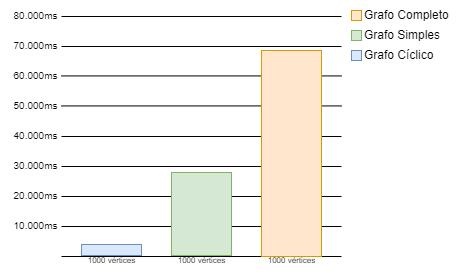
\includegraphics[scale=0.75]{figuras/grafico.png}
\end{center}




\subsection{\esp Regressão}

\begin{figure}[ht]
	\centering	
	\caption[\hspace{0.1cm}Grafo nº vértices x tempo de execução.]{Grafo do nº de vértices x tempo de execução (ms)}
	\vspace{-0.4cm}
	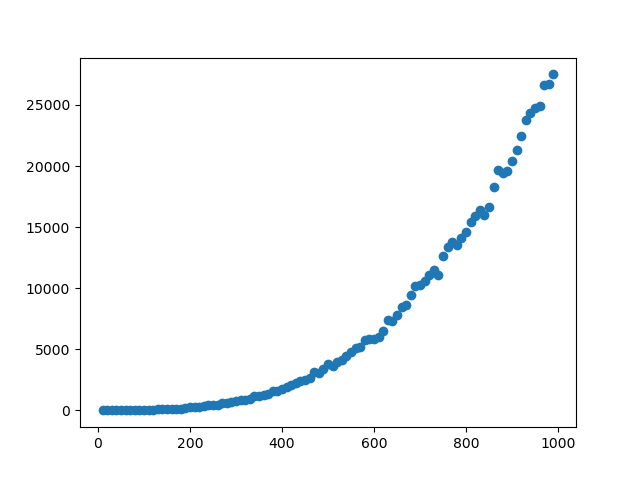
\includegraphics[width=0.6\textwidth]{figuras/complexidade.png}
	 \vspace{-0.2cm}
	\label{fig:figura4}
\end{figure}

A figura acima representa um gráfico do número de vértices pelo tempo de execução. Para encontrarmos a complexidade de tempo do programa, realizamos o teste com vários grafos simples de tamanhos diferentes. Geramos os grafos com tamanhos incrementais de 10 a 10, gerando de tamanho 10 à 990, com a probabilidade de existir aresta entre dois vértices quaisquer igual à 50\%.
A função encontrada na regressão para o tempo de execução (em milisegundos) de acordo com o número de vértices foi de $T(n) = 0.04293861x^2 - 17.17452933x$, com um coeficiente muito preciso de $R^2 = 0.995024467$. Com isso, podemos dizer que nosso programa possui complexidade de tempo quadrática.

\subsection{\esp Conclusão}
O programa roda com uma complexidade de $O(n^{2})$. Por utilizarmos o corte do grafo encontrado com o algoritmo de Edmonds-Karp, a complexidade é reduzida em um grau de magnitude - o pior caso é em grafos completos, onde o número de arestas é reduzido de $n*(n-1)/2$ para $2n - 3$. Por conseguirmos parar a execução do método de força-bruta ao encontrarmos um conjunto de caminhos disjuntos com o mesmo valor do fluxo máximo, o algoritmo também é mais rápido em casos médios. 



%%%%%%%%%%%%%%%%%%%%%%%%%%%%%%%%%%%
%% FIM DO TEXTO
%%%%%%%%%%%%%%%%%%%%%%%%%%%%%%%%%%%

% \selectlanguage{brazil}
%%%%%%%%%%%%%%%%%%%%%%%%%%%%%%%%%%%
%% Inicio bibliografia
%%%%%%%%%%%%%%%%%%%%%%%%%%%%%%%%%%%


\end{document}


